\documentclass[]{article}
\usepackage{graphicx}
%opening
\title{CLRS Exercise}
\author{Tongda Xu}

\begin{document}

\maketitle


\section{15}

\section{15.1-1}
$2^n -1 = \Sigma_{j = 0}^{n-1} 2^j $
\section{15.1-2}
Do not know how!

\section{15.1-3}
See Code

\section{15.1-4}
See Code

\section{15.1-5}
See Code

\section{15.2-1}
See Code

\section{15.2-2}
See Code

\section{15.2-3}

Assume that $\forall k \le n-1, T(k) \ge c2^k$\\
Then $T(n) = \Sigma_{k = 1}^{n-1} T(k)T(n-k) = (n-1)c^22^n > c2^n$\\
So $T(n) = \Omega (n), \omega(n)$

\section{15.2-4}
See Figure ~\ref{fig:15.2-4}

\begin{figure}
	\centering
	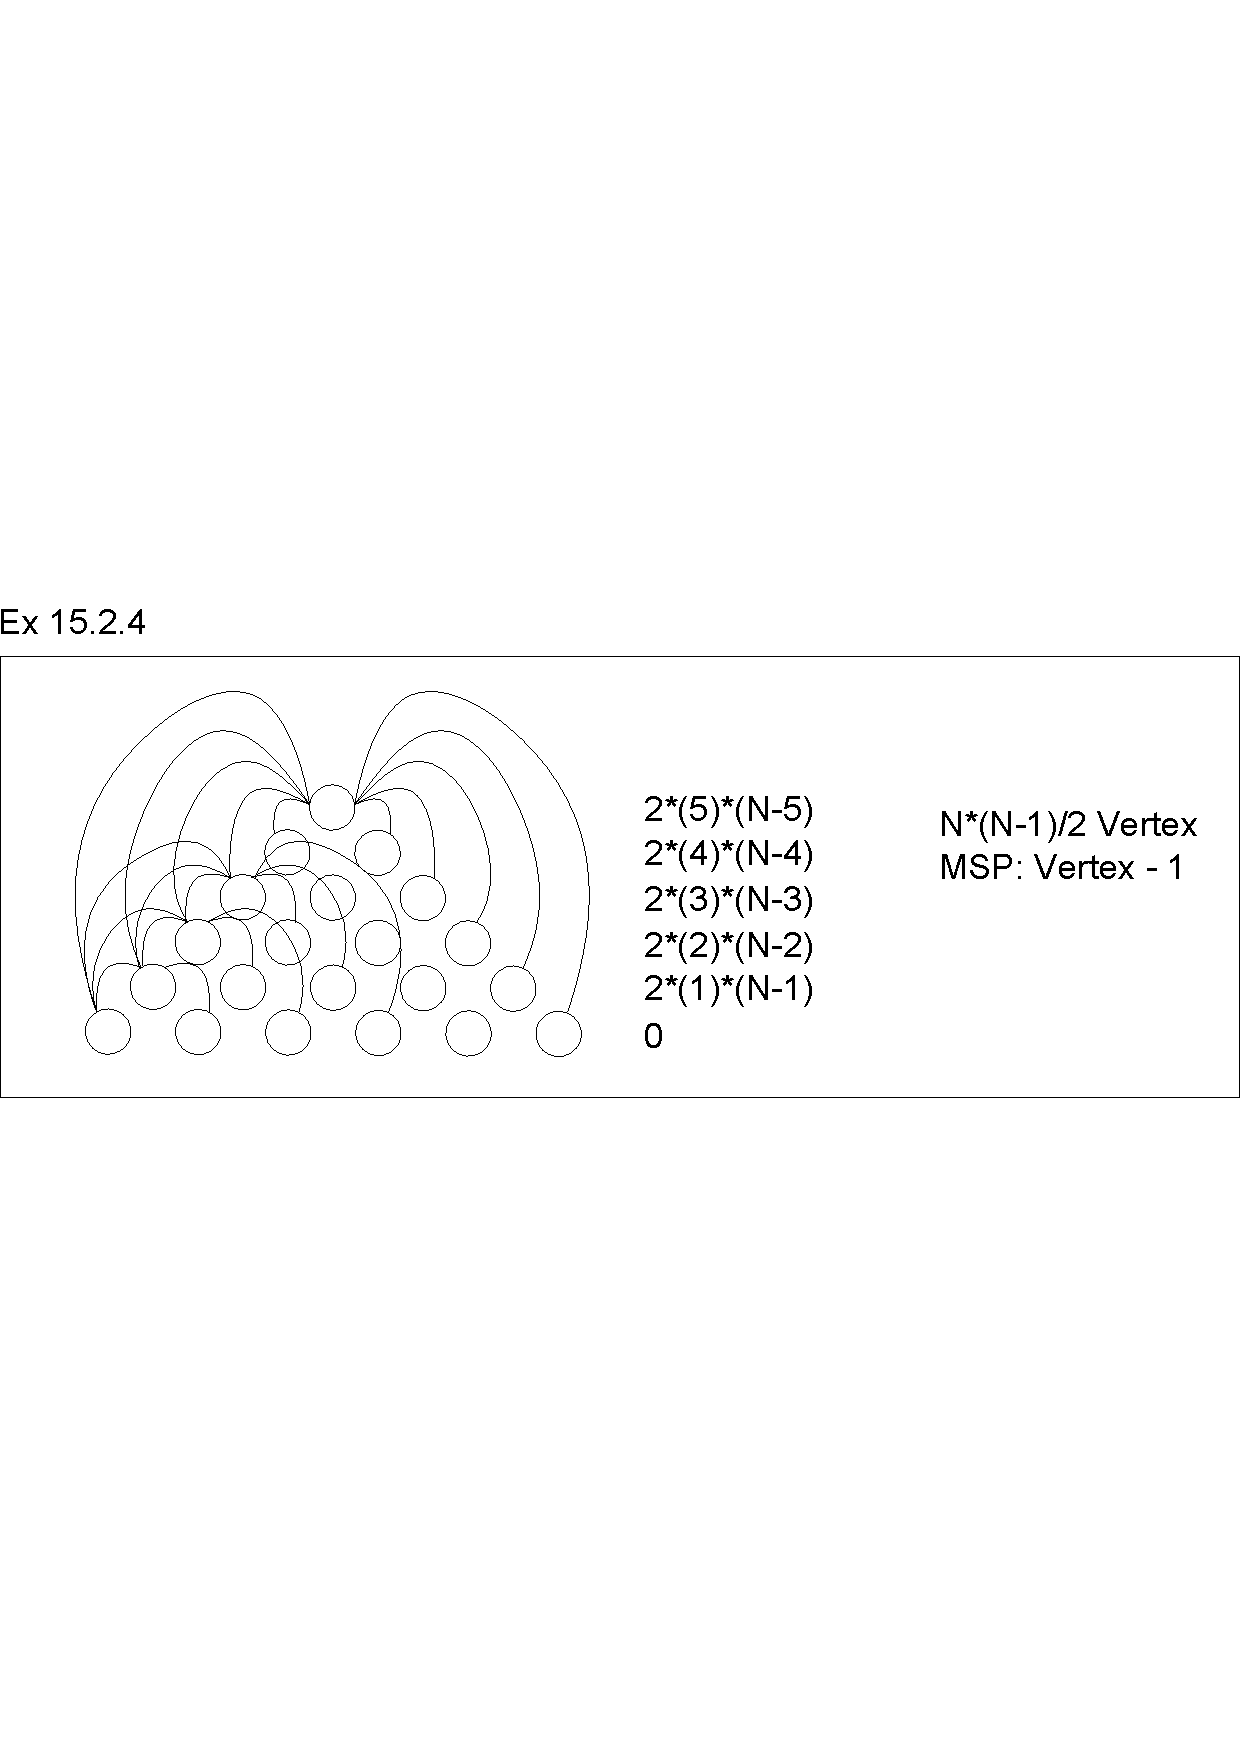
\includegraphics[width=0.8\linewidth]{1524}
	\caption{15.2-4}
	\label{fig:15.2-4}
\end{figure}

\section{15.2-5}
For each level $h(i) = i (n-i)$\\
For tree $T(n) = 2\Sigma_{i = 1}^{n-1}i(n-i)
\\ = \frac{3n^3 + 3n^2}{3} - \frac{2n^3 + 3n^2 +n}{3}
\\ = \frac{n^3 - n }{3}$

\section{15.2-6}
Assume that $\forall k \le n-1, N(k) = k-1$\\
Then $N(n) = N(n-1) + 1$\\
So $N(n) = n-1$


\end{document}
